\documentclass[10pt,a4paper,onecolumn]{article}
\usepackage[usenames,dvipsnames]{color}
\usepackage[colorlinks,citecolor=blue]{hyperref}
\usepackage{appendix}
% we need umlauts in the refs
\usepackage[english]{babel}
\usepackage[utf8]{inputenc}
\usepackage[T1]{fontenc}

%\usepackage[natbib=true,style=authoryear,backend=biber]{biblatex}
\usepackage{authblk}
\renewcommand\Affilfont{\itshape\small}
\usepackage{graphicx}
\usepackage[authoryear]{natbib}
\usepackage{url}
\usepackage{todonotes}
%\usepackage{endfloat}
% nicer units
\usepackage{units}
% better tables
\usepackage{booktabs}
% Some colorings for the tables
%\usepackage[table]{xcolor}

%\usepackage{multirow}

% switch for final stage
%\graphicspath{{pics/}}
\graphicspath{{pics/}
              {pics/generated/}}

%\usepackage{lineno}
%\usepackage[leftbars]{changebar}
%\setlength\changebarsep{0.5em}
%\usepackage{comment}

%\usepackage[space]{grffile}
%\usepackage{latexsym}
%\usepackage{amssymb}
%\usepackage{fancyref}
\usepackage{textcomp}

\usepackage{marvosym}
\usepackage{listings}

\lstset{prebreak=\Righttorque}
\lstset{postbreak=\Lefttorque}
\lstset{breakindent=0pt}
\lstset{frame=lines}
\lstset{aboveskip=4mm}
\lstset{breaklines=true, breakatwhitespace=false}
\urlstyle{same}
% howto cite projects
\newcommand{\purl}[2]{#1\footnote{\url{#2}}}

\newcommand{\sevenT}{\unit[7]{Tesla}}
\newcommand{\threeT}{\unit[3]{Tesla}}
\newcommand{\mm}[1]{\unit[#1]{mm}}
\newcommand{\seconds}[1]{\unit[#1]{s}}

\newcommand{\ie}[0]{\emph{i.e.},\ }
\newcommand{\eg}[0]{\emph{e.g.},\ }
\newcommand{\etc}[0]{\emph{etc.}}


\begin{document}
\bibliographystyle{unsrtnat}
\title{Decoding musical genre with an fMRI encoding model of musical
features -- a 3T/7T comparison}


\author[1]{Moritz~Boos}
\author[2]{J.~Swaroop~Guntupalli}
\author[1]{Cristiano Micheli}
\author[1]{Jochem Rieger}
\author[3,4]{Michael~Hanke}

\affil[1]{Oldenburg, Germany}
\affil[2]{Department of Psychological and Brain Sciences,
  Dartmouth College, Hanover, New Hampshire, USA}
\affil[3]{Psychoinformatics lab, Department of Psychology II, University of
Magdeburg, Magdeburg, Germany}
\affil[4]{Center for Behavioral Brain Sciences, Magdeburg, Germany}
\maketitle
\thispagestyle{fancy}

\listoftodos

\begin{abstract}
% Abstracts should be up to 300 words and provide a succinct summary of the
% article. Although the abstract should explain why the article might be
% interesting, care should be taken not to inappropriately over-emphasise the
% importance of the work described in the article. Citations should not be used
% in the abstract, and the use of abbreviations should be minimized.

\todo[inline]{write abstract}
\end{abstract}

\clearpage


\section*{Introduction}

In functional magnetic resonance imaging (f{MRI}) research, voxel-wise encoding
models are an increasingly popular tool to characterize the
relationship between a real world stimulus and BOLD activity patterns
\citep{NG11,TD+06,KG+08,SZ09}.
Yet not all encoding models are made alike, and a researcher has many degrees
of freedom in constructing one.
Parameters of the data analysis, as well as parameters of BOLD-acquisition, like field strength and resolution,
might impact encoding performance \citep{KB07,FK12}. \citet{SF14} offer some evidence that an
encoding model performs better on 7-Tesla than 3-Tesla data, although differing
number of stimuli are a potential confound.
Even less is known about effects of feature selection strategies or how
the different ways to validate an encoding model relate to each other. \todo[inline]{How about adding
citations used in the next paragraph? There is a new Neuroimage paper from 
Naselaris as well.-Swaroop}

Previous studies have introduced several different measures for the quality of an
encoding model: \citet{ML08} used a binary retrieval task --- checking whether an encoding model's predictions
can be used to identify a stimulus from a pair of stimuli ---
to validate the predicted f{MRI} images for the meaning of nouns. \citet{KG+08} used stimulus
identification, and \citet{NG09} used stimulus reconstruction,
as a metric for encoding performance. In auditory neuroscience, where encoding models are less
frequent, only binary retrieval accuracy \citep{CTK+2012} and stimulus
identification \citep{SF14} have been used.

Recently, a 3-Tesla f{MRI} study on the perception of
musical genres \citep{CTK+2012} has been replicated with 7-Tesla data
\citep{HDH+2015}, making it possible to directly compare the effect of field
strength on data analysis parameters and validation strategies for encoding models. In this study,
we apply three different approaches to encoding validation --- binary retrieval accuracy \citep{ML08},
stimulus identification \citep{KG+08,SF14} and the decoding accuracy of a
stimulus's music genre, and compare them in a 3-Tesla and 7-Tesla dataset with
identical stimuli and comparable design for different analysis strategies.


\section*{Methods}

\subsection*{Stimuli}

Stimuli were five natural, stereo, high-quality music stimuli (\unit[6]{s}
duration; \unit[44.1]{kHz} sampling rate) for each of five different musical
genres: 1) Ambient, 2) Roots Country 3) Heavy Metal, 4) 50s Rock'n'Roll, and 5)
Symphonic. Previously, all 25 stimuli and have been made publicly available \citep{HDH+2015}.

\subsection*{fMRI data}

The analyses presented here were performed on two independently recorded, and
previously published datasets \citep{CTK+2012,HDH+2015} . While these datasets
have been acquired using identical stimuli, with the same number of acquisition
runs and number of stimulation trials, they nevertheless differ in their
precise stimulation timing, stimulation setup and equipment, as well as other
acquisition details. A brief description of both datasets is provided below.
For more information the reader is referred to the respective publications.

\paragraph{\unit[3]{Tesla}}
%
Participants were scanned in a Philips Intera Achieva scanner with 32 channel
SENSE head coil at the Dartmouth College. Functional scans were acquired with
an echo planar imaging sequence (\unit[2]{s} TR; \unit[35]{ms} TR,
90\textdegree flip angle) at \unit[3]{mm} isotropic voxels.
% MIH: as it was published before we probably don't have to include this
%All subjects consented in accordance with the procedures set by the Committee
%for the Protection of Human Subjects at the Dartmouth College. 

Each subject participated in eight functional runs. Stimuli were presented in
an event-related design with a variable trial duration. Each run consisted of a
total of 29 trials corresponding to 25 music clips and 4 catch trials presented
randomly during each run. Each trial started with a \unit[6]{s} of music clip
followed by \unit[4-8]{s} of fixation. For catch trials, a question appeared
after the audio presentation asking whether a particular feature is present in
the music clip such as vocals, guitar, etc. Subjects responded “Yes” or “No”
with a button box. Catch trials helped keep the subjects’ attention to the
music and were discarded from the analyses. Each run had \unit[4]{s} of
fixation at the beginning and \unit[10]{s} of fixation at the end. For further
details, see \citet{CTK+2012}

\paragraph{\sevenT}
%
The procedures for the \unit[7]{Tesla} acquisition were highly similar and only
criticial differences are reported here. Echo-planar BOLD images
(gradient-echo, \unit[2]{s} repetition time (TR), \unit[22]{ms} echo time,
\unit[0.78]{ms} echo spacing, GRAPPA acceleration factor 3) were acquired using
a whole-body \sevenT\ Siemens MAGNETOM magnetic resonance scanner equipped with
a 32 channel brain receive coil. 36 axial slices (thickness \unit[1.4]{mm},
\unit[1.4 $\times$ 1.4]{mm} in-plane resolution) with a 10\% inter-slice gap
were recorded in ascending order.  Slices were oriented to include the ventral
portions of frontal and occipital cortex while minimizing intersection with the
eyeballs. The field-of-view was centred on the approximate location of Heschl's
gyrus.

Instead of dedicated catch trials, similar catch questions as for the 3T
acquisition were presented \unit[4]{s} after the end of the stimulus in
trials with an \unit[8]{s} inter-stimulus delay. Consequently, each run
consisted of 25 trials, and no trials were discarded from the analysis.  There
was no additional fixation at the start of a run. For further details, see
\citet{HDH+2015}, and \citet{HBI+14} for details on MRI acquisition methods.


\subsection*{Preprocessing}

Temporal lobe masks for each participant were extracted from Montreal
Neurological Institute coordinate space using FSL \citep{SJB+04,JBB+12}, and
projected into the subject-specific coordinate system.
Each voxel inside the temporal lobe mask was run-wise $Z$-scored and linearly
de-trended using PyMVPA \citep{HHS09b}. 

\subsection*{Encoding model}

To build an encoding model with high predictive power, we need to find an
appropriate feature representation of the music stimuli.  \citet{CTK+2012}
already compared different feature representations of the same stimuli in the
3-Tesla dataset. They found features corresponding to the timbre of the stimulus
showed the highest binary retrieval accuracy.
We chose a similar feature set made available by \citet{HDH+2015}, the low-quefrency
mel-frequency spectrum (LQ-MFS) of the stimulus.

\begin{figure}
  \centering
  \includegraphics[width=\linewidth]{pics/encoding_scheme}

  \caption{A schematic overview of the encoding process. The spectrogram for
	  each stimulus is transformed into its low-quefrency mel-frequency
	  spectrum (LQ-MFS). Then, the encoding features are extracted by a
  sliding window from the LQ-MFS. Using these features, encoding model is trained on all runs in
  the training set, and used to predict the BOLD activity of the left-out run.
  These predictions are subsequently used for validation.}

 \label{fig:encoding_scheme}
\end{figure}


For each f{MRI} sample $y_{vt}$ (where $t=1,2,..,T$ denotes the time-points and
$v=1,2,..,V$ denotes the voxels) the LQ-MFS features $x_{t}$ $[1\times\widetilde{M}]$
(where $\widetilde{M}$ is the number of LQ-MFS coefficients) of the
corresponding two second part of the stimulus were computed. In case there was
no stimulus presented at time-point $t$, a zero vector $[1\times\widetilde{M}]$ was
used. 

Since the BOLD response is delayed,  the most recent feature vector was removed
for each f{MRI} sample (since it could not yet have influenced the BOLD
activity), and the new feature vector at time-point $t$ was created by
concatenating the prior feature vectors $x_{t-1}$,$x_{t-2}$ and $x_{t-3}$
(see Figure \ref{fig:encoding_scheme}). From
now on, we denote this stacked feature vector as $x_{t}$.
Feature vectors (and the corresponding f{MRI} sample) were removed from the
analysis, if two-thirds or more of the concatenated feature vectors were
zero-vectors.

The BOLD activity time-series, as well as the feature time-series, were
vertically stacked, resulting in a matrix of features $X$ $[N\times M]$ (where $N$ is
the number of f{MRI} samples, and $M$ is number of LQ-MFS coefficients, with
$M=3\widetilde{M}$) and a matrix of BOLD activity $Y$ $[N\times V]$ (where $V$ is
the number of voxels).

This lagging of the stimulus allows us to train the encoding model to predict
the f{MRI} time-series without explicitly modelling the BOLD response.

%probabilistic or objective function minimization, also cite someone about using lin. reg. in encoding
The encoding model could then be expressed as the probability to observe the BOLD activity at time-point $t$ and voxel $v$:
%
\begin{equation}
  \label{eq:encmo}
  p(y_{vt}|x_{t}) = N(y_{vt};x_{t}\beta_{v},\sigma)
\end{equation}
%
where $N(y;\mu,\sigma)$ denotes the probability density at point $y$ for a
Gaussian with mean $\mu$ and standard deviation $\sigma$, and $\beta_{v}$ is a
$[M\times1]$ vector of regression coefficients specific to voxel $v$. To reduce
over-fitting, the regression-coefficients were estimated using ridge regression
\citep{HK70}.  Independently for each voxel, the regularization parameter
$\lambda$ with the lowest mean squared error in a generalized leave-one-out
cross-validation \citep{GHW79} was chosen from a set of candidate values.

\subsection*{Quality metrics} 

\paragraph{Binary retrieval accuracy}

Binary retrieval accuracy \citep{ML08} tests if an encoding model's predictions
can differentiate a stimulus's observed BOLD activity from the BOLD activity
of a decoy stimulus.
Specifically, a stimulus pair is counted as succesfully classified, if the cosine similarity between predicted and
observed f{MRI} responses is greater for the correctly matched predictions and
observations than for the incorrectly matched ones (i.e. the similarity of the observed response of
stimulus A with the predictions for stimulus B and vice versa).
The correct matches for all pair-wise combinations of stimuli, including stimuli from the
same genre, are counted and then divided by the number of combinations.

\paragraph{Matching score}
%
An alternative measure of encoding performance is the correlation rank score or
matching score \citep{SF14}. For each stimulus label $l_{n}$ in the validation set,
its predicted BOLD activity $\widetilde{y}_{n}$ is correlated with the
observed BOLD activity of every stimulus, $y_{i}$ for $i=1..25$. These
correlations are then ordered, and the  matching score $m(l_{n})$ is \[
m(l_{n}) = 1-\frac{rank(l_{n})-1}{N-1} \] Where $rank(l_{n})$ is the rank of
the correlation between predicted $\widetilde{y}_{n}$ and observed $y_{n}$
BOLD activity of $l_{n}$. Finally, the matching scores for all stimuli in the
validation set are averaged.



\begin{figure}
  \centering
  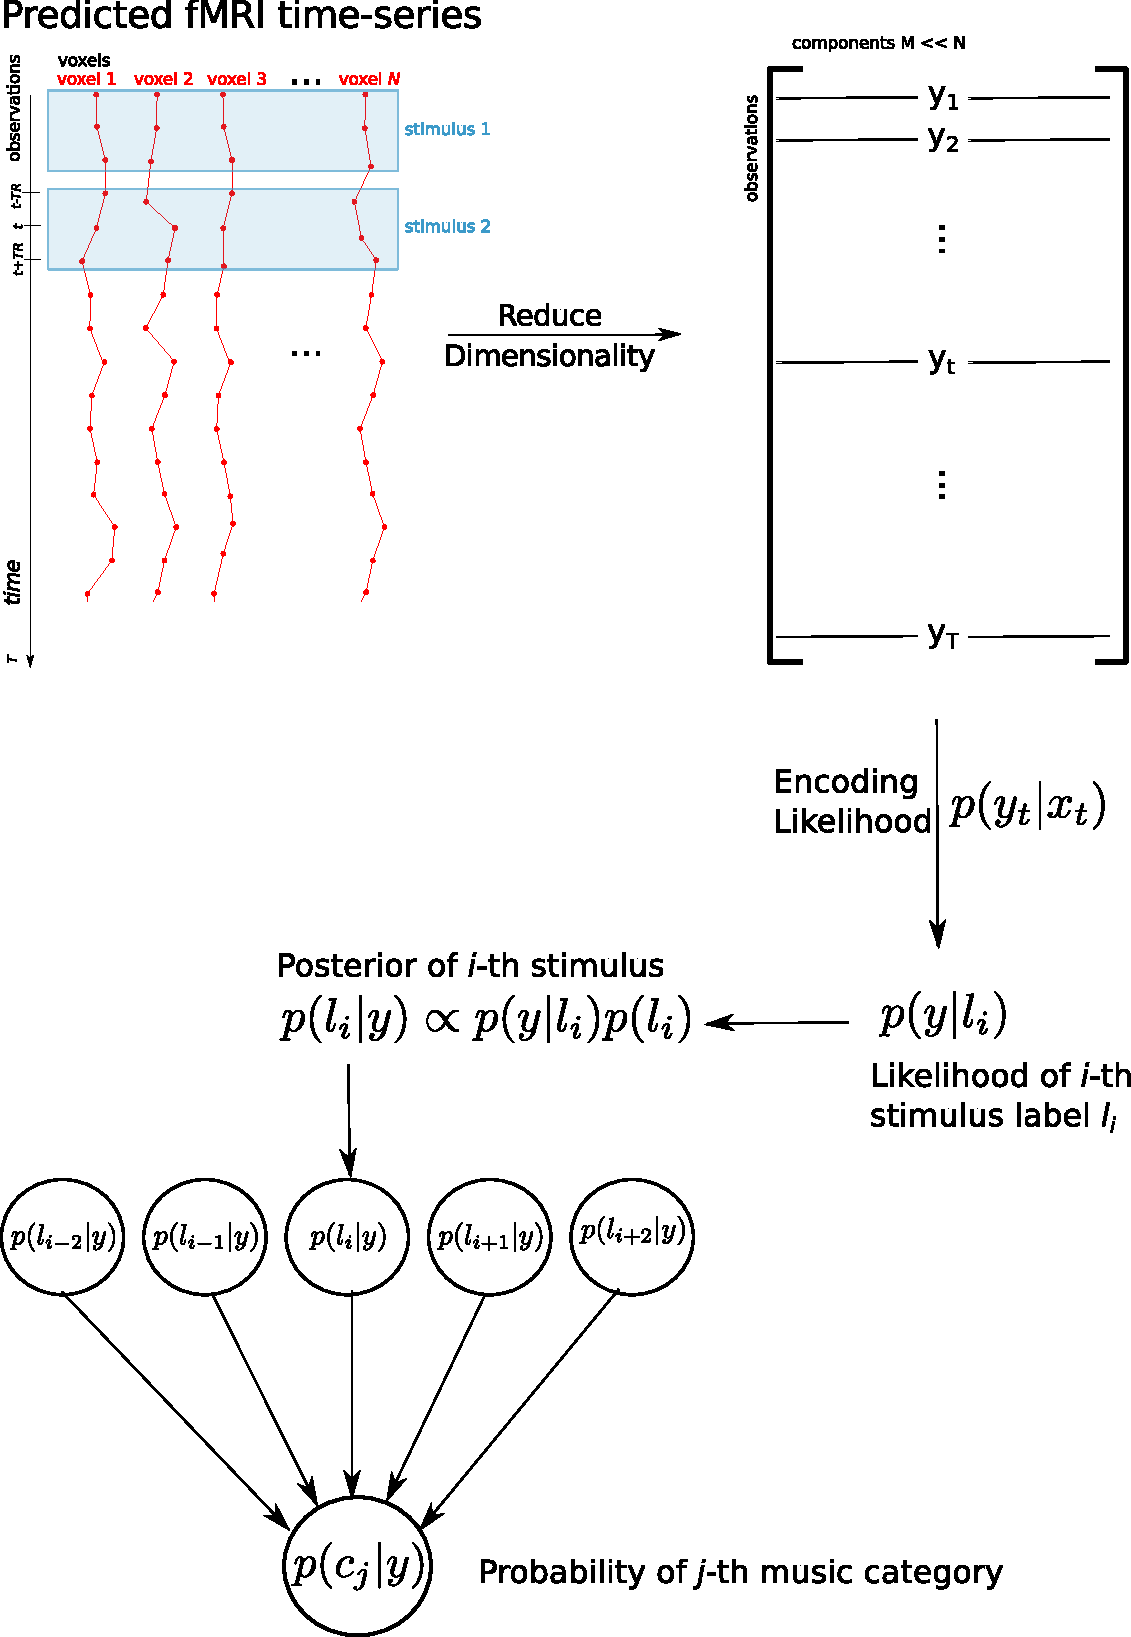
\includegraphics[width=\linewidth]{pics/Decoding_scheme}

  \caption{A schematic overview of the decoding of music category. The predicted
  f{MRI} time series of the validation run is reduced in dimensionality by
  principal component analysis,
  and a multivariate-normal likelihood function $p(y_{t}|x_{t})$ is constructed.
  From there, the probability distribution over music stimuli and subsequently musical categories is estimated.}

 \label{fig:decoding_scheme}
\end{figure}


\paragraph{Decoding of stimulus category}

Instead of testing the encoding performance, we can also test the performance of
a decoder based on the individual encoding models \citet{NG11}
(Figure \ref{fig:decoding_scheme}). To go from
$p(y_{vt}|x_{t})$ to $p(x_{t}|y_{t})$ we follow \citet{NG09} and first condense
the large number of voxel-specific encoding models into one multi-voxel encoding model.
To do this we project the predicted and observed f{MRI} data onto the first $k$
principal components of the $[N\times V]$ matrix of predicted BOLD activity, where $k$ is the number of principal components that maximize the decoding
accuracy on the training set for this participant.
As in \citet{NG09} we construct the $k$-dimensional multivariate normal
probability density function $p(y_{t}|x_{t})$ to obtain a likelihood function across voxels.
To build a decoding model, we now express this likelihood in terms of the label
of the music stimulus, instead of its LQ-MFS features.
We use the simplifying assumption that the BOLD activity is influenced by the music stimuli only through their LQ-MFS
coefficients $x$, and --- given that each music stimulus was associated with only
three (lagged) LQ-MFS representations --- the likelihood to observe a given
triple of consecutive $y$ for a specific music stimulus $l_{i}$ is $p(y|l_{i}) \propto
p(y_{t-1}|x_{1})p(y_{t}|x_{2})p(y_{t+1}|x_{3})$ where $t$ is the sample 6
seconds after the start of the music stimulus and $x$ are the three LQ-MFS
feature vectors of this stimulus.
For a given triple of consecutive BOLD activity $y$ from the same stimulus, we can now estimate the probability distribution over music stimuli
$p(l_{i}|y)$ (for $i=1..25$) by using Bayes' rule: $p(l_{i}|y) \propto
p(y|l_{i})p(l_{i})$ and ignoring the normalizing constant $p(y)$. Since each
stimulus was presented was presented exactly once, it has an uniform prior
distribution with $p(l_{i})=\frac{1}{25}$. The mode of this distribution is the
most probable presented stimulus given the data.
We can then decode the musical genre of the presented stimulus given the observed BOLD activity as the mode of $p(c_{i}|y)
\propto \prod\nolimits_{l \in stim(c_{i})} p(l|y)$ where $stim(c_{i})$ are
the labels of the stimuli belonging to the genre $c_{i}$. 

\subsection*{Voxel selection}

We varied the number of voxels used in the analysis, both for 3- and 7-Tesla f{MRI} data,
and selected which voxels to keep by two different criteria. Both criteria were
based on voxel characteristics in the training set.  

\paragraph{Selection by stability}

\citet{ML08} selected the 500 most stable voxels for their analysis. For a
single voxel, each run can be represented as a vector of BOLD activity, where each
entry is associated with one stimulus. A voxel's "stability score" is then the
average (pair-wise) correlation between the vectors of the eight runs for all
combinations of runs.
This criterion selects voxels with consistent activation for each stimulus across runs.

\paragraph{Selection by $r^2$}

Since we are interested in encoding performance, we can use the quality of
predictions of each voxel's encoding model as a selection criterion. We compute
the coefficient of determination $r^2$ for each voxel-specific encoding model in
the training set. Using this criterion selects voxels whose activity can be explained well
by an LQ-MFS-based encoding model.

\section*{Results}

We varied the number of voxels used in the analysis and how they were selected,
both for 3- and 7-Tesla f{MRI} data, and compared the resulting differences in
three encoding metrics. To differentiate between effects of voxel number and
overall volume of the voxels, which differs in 3- and 7-Tesla, we show the results as a function of the number of voxels, as well as overall volume of
these voxels.

\begin{figure}
  \centering
  \def\svgwidth{\linewidth}
  \input{pics/binary_score_joint.pdf_tex}
	
  \caption{\textbf{A} Mean binary retrieval accuracy as a function of the included number of
  voxels for 3- and 7-Tesla, for stability- and $r^2$-based voxel selection. Error bars denote the bootstrapped 95\% confidence
  interval of the mean. The mean is taken over binary retrieval accuracies of
  eight runs for each of the 19 participants. \textbf{B} Mean binary retrieval accuracy as a function of the overall volume of
	  the included voxels for 3- and 7-Tesla, for stability- and $r^2$-based voxel selection.}

 \label{fig:binary_retrieval}
\end{figure}

\subsection*{Binary retrieval accuracy}

Differences in binary retrieval accuracy are shown in Figure \ref{fig:binary_retrieval}. For both selection criteria, binary retrieval
accuracy is higher in 3-Tesla than 7-Tesla data for lower numbers of voxels.
When a higher number of the most stable voxels are included, binary retrieval accuracy increases for 7-Tesla data, while decreasing for 3-Tesla data.    
In contrast, increasing the number of voxels included by $r^2$ decreases the
binary retrieval accuracy for 3-Tesla, as well as 7-Tesla data, although the
decrease seen in 3-Tesla data is larger. The peak
performance of 3-Tesla as well as 7-Tesla encoding models, is higher using
voxels selected by their $r^2$.
Indexing by the overall volume of the voxels, reveals a very similar, but
shifted, pattern for 3- and 7-Tesla data.

\begin{figure}
  \centering
  \def\svgwidth{\linewidth}
  \input{pics/matching_score_joint.pdf_tex}
	
  \caption{\textbf{A} Mean matching score as a function of the included number of
  voxels for 3- and 7-Tesla, for stability- and $r^2$-based voxel selection. Error bars denote the bootstrapped 95\% confidence
  interval of the mean. The mean is taken over binary retrieval accuracies of
  eight runs for each of the 19 participants. \textbf{B} Mean matching score as a function of the overall volume of
	  the included voxels for 3- and 7-Tesla, for stability- and $r^2$-based voxel selection.}

 \label{fig:matching_score}
\end{figure}

\subsection*{Matching score}

In Figure \ref{fig:matching_score}, the matching score is shown. Again, for
few voxels, encoding models for 3-Tesla data produce a higher score than encoding
models for 7-Tesla data. Increasing the number of voxels increases the matching
score for 7-Tesla data, and decreases the score for 3-Tesla data. This pattern
is present in both selection criteria. For voxels selected by $r^2$, there is a
steeper increase and decrease and a higher peak for both field strengths.
If indexed by the overall voxel volume, similarities in the overlapping regions
of the 3- and 7-Tesla matching score curves can be seen.
\begin{figure}
  \centering
  \def\svgwidth{\linewidth}
  \input{pics/decoding_accuracy_joint.pdf_tex}
	
  \caption{\textbf{A} Mean decoding accuracy of music category as a function of the included number of
  voxels for 3- and 7-Tesla, for stability- and $r^2$-based voxel selection. Error bars denote the bootstrapped 95\% confidence
  interval of the mean. The mean is taken over binary retrieval accuracies of
  eight runs for each of the 19 participants. \textbf{B} Mean decoding accuracy
  of music category as a function of the overall volume of the included voxels for 3- and 7-Tesla, for stability- and $r^2$-based voxel selection.}
 \label{fig:decoding_accuracy}
\end{figure}


\subsection*{Decoding accuracy}

The decoding accuracy of each stimulus's music category is shown in Figure
\ref{fig:decoding_accuracy}. Since the decoder is based on an encoding model, a
natural comparison is with the performance of a standard decoder. For both selection methods, we contrast the decoding
performance of the encoding model with the decoding performance of a linear Support
Vector Machine (SVM) \citep{FCH+08,V13}. While such a decoder can use the subset of the most stable voxels, it can only select the voxels with the highest $r^2$, if it leverages the information of an encoding model. We still include these data, to show which information could be extracted from these voxels by a more sophisticated decoding approach.  The decoding accuracy was higher for 7-Tesla data than for 3-Tesla data, across all voxel numbers and selection criteria.  Selecting the most stable voxels, the decoding accuracy slightly increases for 7-Tesla data with higher numbers of voxels, while decreasing for 3-Tesla data.
If we select the voxel-specific encoding models with the highest $r^2$, the
decoding accuracy decreases for 3-Tesla data, but first stays level and then
decreases for 7-Tesla data. Encoding models on 3-Tesla data show a higher or equal decoding accuracy than a discriminative decoder across all numbers of
voxels. This contrasts the pattern present in the 7-Tesla data, where our
decoding model shows a higher decoding accuracy only for smaller numbers of
voxels. %Using voxels selected by $r^2$ the Support Vector Machine starts to
%outperform the encoding model for lower numbers of voxels.

\begin{figure}
  \centering
  \def\svgwidth{\linewidth}
  \input{pics/binary_score_joint_mve.pdf_tex}
	
  \caption{\textbf{A} Mean binary retrieval accuracy for a single encoding model as a function of the included number of
  voxels for 3- and 7-Tesla, for stability- and $r^2$-based voxel selection. Error bars denote the bootstrapped 95\% confidence
  interval of the mean. The mean is taken over binary retrieval accuracies of
  eight runs for each of the 19 participants. \textbf{B} Mean binary retrieval
  accuracy for a single encoding model as a function of the overall volume of
	  the included voxels for 3- and 7-Tesla, for stability- and $r^2$-based voxel selection.}

\label{fig:binary_retrieval_mve}
\end{figure}

\begin{figure}
  \centering
  \def\svgwidth{\linewidth}
  \input{pics/matching_score_joint_mve.pdf_tex}
	
  \caption{\textbf{A} Mean matching score for a single encoding model as a function of the included number of
  voxels for 3- and 7-Tesla, for stability- and $r^2$-based voxel selection. Error bars denote the bootstrapped 95\% confidence
  interval of the mean. The mean is taken over binary retrieval accuracies of
  eight runs for each of the 19 participants. \textbf{B} Mean matching score for a single encoding model as a function of the overall volume of
	  the included voxels for 3- and 7-Tesla, for stability- and $r^2$-based voxel selection.}

 \label{fig:matching_score_mve}
\end{figure}

\subsection*{Effect of Multi-Voxel Encoding}

Field strength affects performance differentially in the binary
retrieval/matching score and the decoding accuracy. Since our decoding scheme
had two parts -- reducing the independent voxel-wise encoding models to a single
encoding model (1) and computing the posterior probability of a stimulus given
the observed f{MRI} data (2) -- we cannot claim what causes this difference.

Therefore, we estimated the binary retrieval accuracy
\ref{fig:binary_retrieval_mve} and the matching score
\ref{fig:matching_score_mve} using the same reduced encoding model as in the decoding accuracy.

\missingfigure{model validation on the movie}

\section*{Discussion}

Our results show considerable variation of different quality metrics with
parameters of the data analysis and BOLD-acquisition. We demonstrate that the
patterns of this variation differ between validation strategies and
that the effects of field strength, voxel selection, and voxel number are
inconsistent across these metrics.

Specifically, we show a similar performance in purely encoding based metrics for 3- and
7-Tesla data with a slightly worse peak performance for 7-Tesla, but observe that this effect is mediated by the number of voxels
used. A previous study \citep{SF14} found a higher performance for 7-Tesla
data for the matching score, although using a different number of stimuli in
the 3- and 7-Tesla datasets. %Furthermore, this study differs in the selection of voxels, the choice of stimulus features and the use
%of an explicit BOLD-model instead of a lagged feature representation.

One possible reason why we see a worse peak performance in these metrics for
higher field strength, might be the increased susceptibility to head-motion
artifacts and physiological noise in a single voxel. \citet{KB07} argue that
challenges posed by high-resolution f{MRI} might be tackled more easily by an
information-based approach, instead of an activation-based one, partly because
neural information can be locally combined without averaging. Since voxels are
treated independently in a voxel-wise encoding model, this advantage is lost if
voxel-specific information is not combined later on. In fact, if we reduce the multi-voxel encoding model
to a single joint encoding model (\citep[see][]{NG09}), we observe a different
pattern for field strength: the obtained decoding accuracy is consistently higher in the 7-Tesla than the 3-Tesla dataset. 
This reduction does only use information captured by the encoding models, it
is estimated from the predictions for a set of voxels, not from the neuronal
response itself, but this combination of voxel-specific information is still
sufficient to make a higher field strength advantageous. 


The number of voxels affect the encoding performance differentially for low
and high field strength. This is not surprising, voxel size differs for the 3-
and 7-Tesla data. Indexing by the overall volume of the selected voxels, instead
of their number, reveals similarities in performance when 3- and 7-Tesla
encoding models are trained on a similar volume. 

Selecting the voxels by $r^2$ instead of a stability criterion, improves
performance especially in the lower number of voxels for the binary retrieval
accuracy and the decoding accuracy, while widening the performance gap between 3- and 7-Tesla
data in the matching score. Including voxels ordered by $r^2$ --- a measure that captures
encoding performance in a single voxel --- gives diminishing returns for higher
numbers of voxels: Voxels for which an encoding model performs well are already
included, and each additional voxel decreases the joint encoding performance.
Interestingly, this pattern is not seen in the matching score, where
performance in 7-Tesla is worse for the smallest number of voxels and increases
with voxel number. The same pattern is seen in the performance of the linear
SVM. Even with information from an encoding model --- selecting voxels by
$r^2$ --- a standard decoder can initially not take advantage of this information
as well as an encoding model. For the high field strength condition, the
decoder improves if more voxels are included and eventually performs better than
the encoding model. This might be an effect of the sheer number of features used by the decoder, or of the information content of these voxels,
i.e. because the decoder profits from pattern information that is not related to
the LQ-MFS features of the stimulus, and would therefore be more present in a
voxel with lower $r^2$ in encoding LQ-MFS.


\section*{Author contributions}
%In order to give appropriate credit to each author of an article, the
%individual contributions of each author to the manuscript should be detailed
%in this section. We recommend using author initials and then stating briefly
%how they contributed.

MB performed the analysis and wrote the manuscript.
JSG contributed to the manuscript.
MH contributed to the manuscript.


\section*{Competing Interests}
No competing interests were disclosed.

\section*{Grant Information}

This research was, in part, supported by the German Federal Ministry of
Education and Research (BMBF) as part of a US-German collaboration in
computational neuroscience (CRCNS; awarded to James Haxby, Peter Ramadge, and
Michael Hanke), co-funded by the BMBF and the US National Science Foundation
(BMBF 01GQ1112; NSF 1129855).  Work on the data-sharing technology employed for
this research was supported by US-German CRCNS project awarded to
Yaroslav~O.~Halchenko and Michael~Hanke, co-funded by the BMBF and the US
National Science Foundation (BMBF 01GQ1411; NSF 1429999).  Michael Hanke was
supported by funds from the German federal state of Saxony-Anhalt, Project:
Center for Behavioral Brain Sciences.


\section*{Acknowledgements}
%This section should acknowledge anyone who contributed to the research or the
%article but who does not qualify as an author based on the criteria provided
%earlier (e.g. someone or an organisation that provided writing assistance).
%Please state how they contributed; authors should obtain permission to
%acknowledge from all those mentioned in the Acknowledgements section.  Please
%do not list grant funding in this section (this should be included in the
%Grant information section - See above).

We are grateful to Michael Casey and the musicians ;) \ldots

\todo[inline]{express gratitude}

\bibliography{references}
\end{document}

% vim: textwidth=80 colorcolumn=81
